\documentclass[border=10pt,transparent]{standalone}
\usepackage{tikz}
\usepackage{amsmath, amssymb}
\usetikzlibrary{arrows.meta,positioning,calc,fit,backgrounds,shapes.geometric,shapes.misc}

\definecolor{quantumcolor}{HTML}{6C1A42}   % Meharry Maroon — quantum pathway
\definecolor{classiccolor}{HTML}{1A6C5E}   % Teal — classical pathway
\definecolor{fusioncolor}{HTML}{C49A2A}    % Gold — fusion layer
\definecolor{outputcolor}{HTML}{2C5F8A}    % Blue — output
\definecolor{lightgray}{HTML}{F5F5F5}

\begin{document}
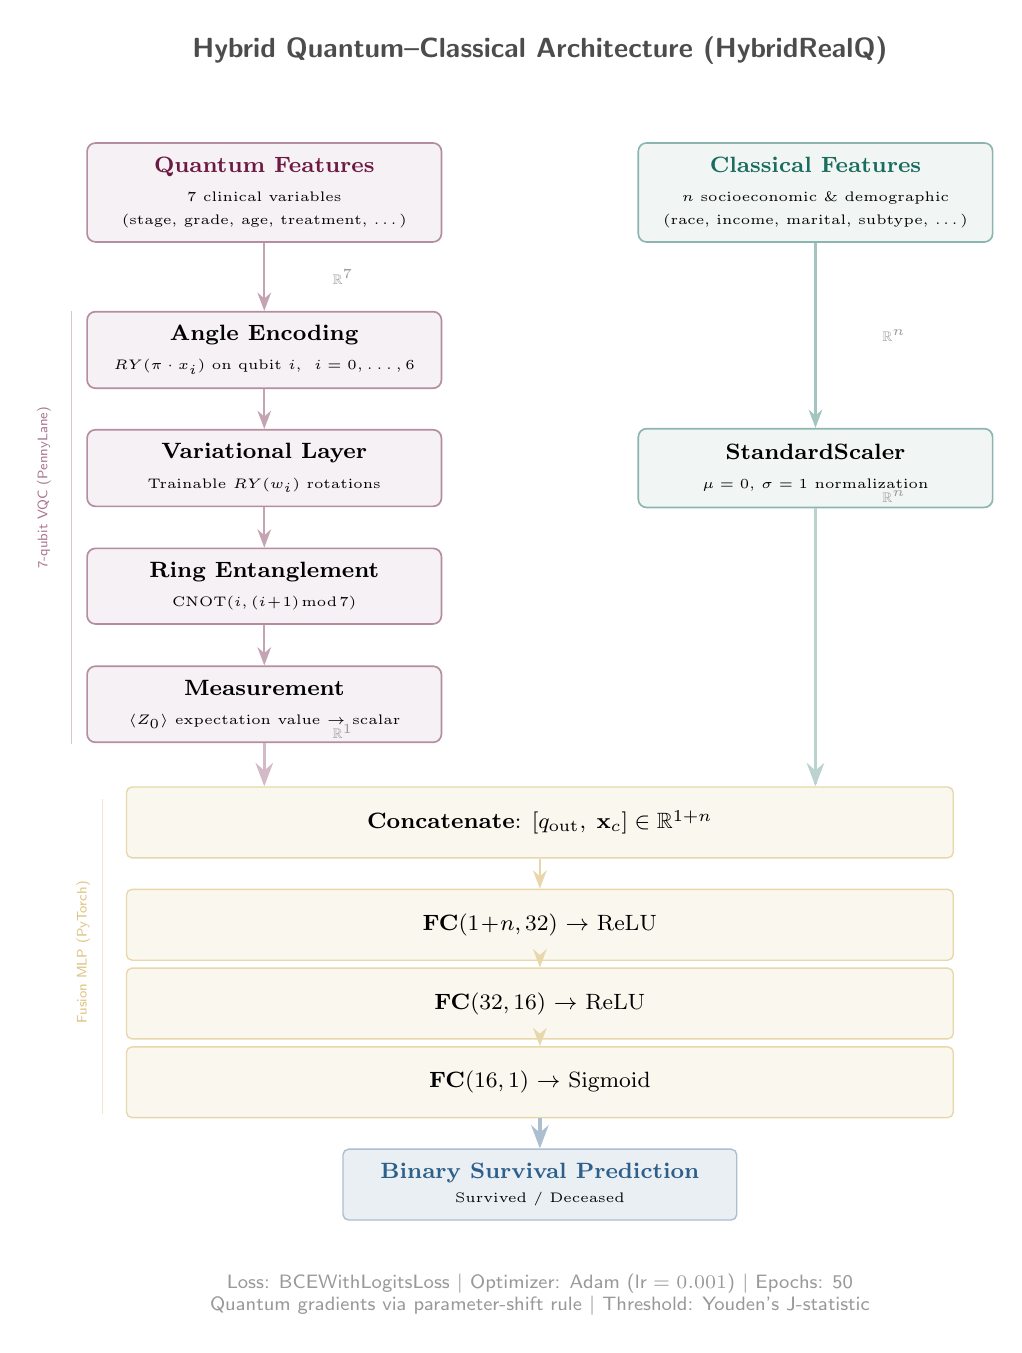
\begin{tikzpicture}[
    box/.style={rectangle, draw=black!60, rounded corners=2pt, font=\footnotesize,
                minimum height=0.85cm, inner sep=5pt, fill=white, line width=0.5pt, align=center},
    qbox/.style={rectangle, draw=quantumcolor!50, rounded corners=3pt, font=\footnotesize,
                 minimum height=0.85cm, inner sep=5pt, fill=quantumcolor!6, line width=0.6pt, align=center},
    cbox/.style={rectangle, draw=classiccolor!50, rounded corners=3pt, font=\footnotesize,
                 minimum height=0.85cm, inner sep=5pt, fill=classiccolor!6, line width=0.6pt, align=center},
    arr/.style={->, >=Stealth, line width=0.8pt, color=black!40},
    thickarr/.style={->, >=Stealth, line width=1.2pt, color=black!50},
    seclbl/.style={font=\normalsize\bfseries\sffamily, text=black!70},
    dimlbl/.style={font=\tiny\sffamily, color=black!40},
]

% ═══════════════════════════════════════════════════════════════
% Title
% ═══════════════════════════════════════════════════════════════

\node[seclbl] at (0, 1.8) {Hybrid Quantum--Classical Architecture (HybridRealQ)};

% ═══════════════════════════════════════════════════════════════
% Input Layer
% ═══════════════════════════════════════════════════════════════

\node[qbox, minimum width=4.5cm, minimum height=1.2cm] (qinput) at (-3.5, 0)
    {\textbf{\textcolor{quantumcolor}{Quantum Features}}\\[1pt]{\tiny 7 clinical variables}\\[-1pt]{\tiny (stage, grade, age, treatment, \ldots)}};

\node[cbox, minimum width=4.5cm, minimum height=1.2cm] (cinput) at (3.5, 0)
    {\textbf{\textcolor{classiccolor}{Classical Features}}\\[1pt]{\tiny $n$ socioeconomic \& demographic}\\[-1pt]{\tiny (race, income, marital, subtype, \ldots)}};

% ═══════════════════════════════════════════════════════════════
% Quantum Pathway (left)
% ═══════════════════════════════════════════════════════════════

\node[qbox, minimum width=4.5cm] (encode) at (-3.5, -2.0)
    {\textbf{Angle Encoding}\\[1pt]{\tiny $RY(\pi \cdot x_i)$ on qubit $i$, \  $i=0,\ldots,6$}};

\node[qbox, minimum width=4.5cm] (varlayer) at (-3.5, -3.5)
    {\textbf{Variational Layer}\\[1pt]{\tiny Trainable $RY(w_i)$ rotations}};

\node[qbox, minimum width=4.5cm] (entangle) at (-3.5, -5.0)
    {\textbf{Ring Entanglement}\\[1pt]{\tiny CNOT$(i, (i\!+\!1)\!\bmod\!7)$}};

\node[qbox, minimum width=4.5cm] (measure) at (-3.5, -6.5)
    {\textbf{Measurement}\\[1pt]{\tiny $\langle Z_0 \rangle$ expectation value $\to$ scalar}};

% Quantum arrows
\draw[arr, color=quantumcolor!40] (qinput.south) -- (encode.north);
\draw[arr, color=quantumcolor!40] (encode.south) -- (varlayer.north);
\draw[arr, color=quantumcolor!40] (varlayer.south) -- (entangle.north);
\draw[arr, color=quantumcolor!40] (entangle.south) -- (measure.north);

% Dimension labels
\node[dimlbl] at ($(qinput.south)!0.5!(encode.north)+(1.0,0)$) {$\mathbb{R}^7$};
\node[dimlbl] at ($(measure.south)+(1.0,0.15)$) {$\mathbb{R}^1$};

% 7-qubit circuit bracket
\node[font=\tiny\sffamily, color=quantumcolor!60, rotate=90] at (-6.3, -3.75) {7-qubit VQC (PennyLane)};
\draw[quantumcolor!25, line width=0.4pt] (-5.95, -1.5) -- (-5.95, -7.0);

% ═══════════════════════════════════════════════════════════════
% Classical Pathway (right) — raw features pass through directly
% ═══════════════════════════════════════════════════════════════

\node[cbox, minimum width=4.5cm, minimum height=1.0cm] (cpass) at (3.5, -3.5)
    {\textbf{StandardScaler}\\[1pt]{\tiny $\mu=0$, $\sigma=1$ normalization}};

% Classical arrow
\draw[arr, color=classiccolor!40] (cinput.south) -- (cpass.north);
\node[dimlbl] at ($(cinput.south)!0.5!(cpass.north)+(1.0,0)$) {$\mathbb{R}^n$};
\node[dimlbl] at ($(cpass.south)+(1.0,0.15)$) {$\mathbb{R}^n$};

% ═══════════════════════════════════════════════════════════════
% Fusion Layer
% ═══════════════════════════════════════════════════════════════

\node[box, fill=fusioncolor!8, draw=fusioncolor!40, minimum width=10.5cm, minimum height=0.9cm]
    (concat) at (0, -8.0)
    {\textbf{Concatenate}: $[q_{\text{out}},\; \mathbf{x}_c] \in \mathbb{R}^{1+n}$};

\node[box, fill=fusioncolor!8, draw=fusioncolor!40, minimum width=10.5cm, minimum height=0.9cm]
    (fc1) at (0, -9.3)
    {\textbf{FC$(1\!+\!n, 32)$} $\to$ ReLU};

\node[box, fill=fusioncolor!8, draw=fusioncolor!40, minimum width=10.5cm, minimum height=0.9cm]
    (fc2) at (0, -10.3)
    {\textbf{FC$(32, 16)$} $\to$ ReLU};

\node[box, fill=fusioncolor!8, draw=fusioncolor!40, minimum width=10.5cm, minimum height=0.9cm]
    (fc3) at (0, -11.3)
    {\textbf{FC$(16, 1)$} $\to$ Sigmoid};

% Fusion arrows
\draw[thickarr, color=quantumcolor!30] (measure.south) -- ++(0,-0.5) -| ($(concat.north)+(-3.5,0)$);
\draw[thickarr, color=classiccolor!30] (cpass.south) -- ++(0,-3.5) -| ($(concat.north)+(3.5,0)$);
\draw[arr, color=fusioncolor!40] (concat.south) -- (fc1.north);
\draw[arr, color=fusioncolor!40] (fc1.south) -- (fc2.north);
\draw[arr, color=fusioncolor!40] (fc2.south) -- (fc3.north);

% Fusion label
\node[font=\tiny\sffamily, color=fusioncolor!60, rotate=90] at (-5.8, -9.65) {Fusion MLP (PyTorch)};
\draw[fusioncolor!25, line width=0.4pt] (-5.55, -7.7) -- (-5.55, -11.7);

% ═══════════════════════════════════════════════════════════════
% Output
% ═══════════════════════════════════════════════════════════════

\node[box, fill=outputcolor!10, draw=outputcolor!40, minimum width=5cm, minimum height=0.9cm]
    (output) at (0, -12.6)
    {\textbf{\textcolor{outputcolor}{Binary Survival Prediction}}\\[-1pt]{\tiny Survived / Deceased}};

\draw[thickarr, color=outputcolor!40] (fc3.south) -- (output.north);

% ═══════════════════════════════════════════════════════════════
% Training details (bottom annotation)
% ═══════════════════════════════════════════════════════════════

\node[font=\scriptsize\sffamily, color=black!40, align=center] at (0, -14.0)
    {Loss: BCEWithLogitsLoss \textbar\ Optimizer: Adam ($\text{lr}=0.001$) \textbar\ Epochs: 50\\
     Quantum gradients via parameter-shift rule \textbar\ Threshold: Youden's J-statistic};

\end{tikzpicture}
\end{document}
